\documentclass[11pt,spanish]{article}

% Paquetes
\usepackage{amstext}
\usepackage{amssymb}
\usepackage{babel}
    \addto\shorthandsspanish{\spanishdeactivate{~<>}}
    \decimalpoint
\usepackage{float}
\usepackage[T1]{fontenc}
\usepackage[a4paper]{geometry}
    \geometry{verbose,tmargin=3cm,bmargin=2cm,lmargin=2.5cm,rmargin=2.5cm}
\usepackage{graphicx}
\usepackage[utf8]{inputenc}
\usepackage{mathptmx}
\usepackage{units}

% tipo de fuente 
\usepackage{lmodern}

\makeatletter

\makeatother


\begin{document}

% Título
    \begin{center}
    \textsc{\large Física 2 (Física) - Cátedra Diana Skigin}
    \par\end{center}{\large \par}
    
    \begin{center}
    \textsc{\large Segundo  Cuatrimestre de 2021}
    \par\end{center}{\large \par}
    
    \begin{center}
    \textsc{\large Guía 2: Sistemas continuos}
    \par\end{center}{\large \par}

% Comienzo 
\begin{enumerate}

\section*{Condiciones de contorno en cuerdas y tubos}

% Ejercicio 1

    \item Se tiene una cuerda de longitud $L$ y densidad lineal de masa $\mu$
    sometida a una tensión $T_{0}$. Proponga como solución de la ecuación
    de ondas para un modo normal a la expresión:
    $\Psi(x,t)=A\sin(kx+\varphi)\cos(\omega t+\theta)$. Tome el sistema de
    coordenadas con $x=0$ en un extremo de la cuerda y $x=L$ en el otro.
    Encuentre la forma particular que adopta la solución propuesta en los
    siguientes casos: 

    \begin{enumerate}
        \item $\Psi(0,t)=\Psi(L,t)=0$ (ambos extremos están fijos).

        \item $\Psi(0,t)=0$ y $\frac{\partial\Psi}{\partial x}(L,t)=0$ (un
        extremo está fijo y el otro está libre). ¿Imponer que un extremo se
        encuentre ``libre'' es equivalente a no imponer condiciones de contorno
        sobre ese extremo? ¿Cómo lograría un extremo ``libre'' para la cuerda? 

        \item $\frac{\partial\Psi}{\partial x}(0,t)=\frac{\partial\Psi}{\partial x}(L,t)=0$
        (ambos extremos se encuentran libres). ¿A qué corresponde el modo de
        frecuencia mínima? ¿Cuánto vale la frecuencia de oscilación de ese modo?

        \item Ahora tome un sistema de coordenadas con $x=0$ en el centro de la
        cuerda. Halle la forma que adopta la solución general propuesta si
        $\Psi(-L/2,t)=\Psi(L/2,t)=0$ (ambos extremos fijos).

    \end{enumerate}

% Ejercicio 2

    \item Se tiene una cuerda de 20 cm de longitud y 5 g de masa, sometida a
    una tensión de 120 N. Calcule sus modos naturales de oscilación. ¿Son todos
    audibles para el oído humano?

% Ejercicio 3

    \item Las cuatro cuerdas de un violín, considere que todas son de igual
    longitud, emiten en su modo fundamental las notas: sol$_{\text{2}}$ (198/s);
    re$_{\text{3}}$ (297/s); la$_{\text{3}}$ (440/s) y mi$_{\text{4}}$ (660/s).
    La primera cuerda es de aluminio ($\rho=2.6$ g/cm$^{3}$ y diámetro
    $d_{1}=0.09\unit{\, cm}$); las dos siguientes son de otro material
    ($\rho=1.2$ g/cm$^{3}$) y diámetros $d_{2}=0.12\unit{\, cm}$ y
    $d_{3}=0.1\unit{\, cm}$, y la cuarta es de acero ($\rho=7.5$ g/cm$^{3}$) y
    diámetro $d_{4}=0.1\unit{\, cm}$. Calcular las tensiones a las
    que deben estar sometidas con respecto a la primera.

% Ejercicio 4

    \item Se tiene un tubo de longitud $L$. Considere las siguientes
    posibilidades: 

    \begin{itemize}
        \item Está cerrado en ambos extremos, lleno de aire en su interior.
        \item Tiene un extremo cerrado y el otro abierto. 
        \item Ambos extremos están abiertos.
    \end{itemize}

    \begin{description}
        \item [{Datos:}] velocidad de propagación de las ondas $v_{s}$, $L$,
        $P_{0}$ (presión atmosférica), $\rho_{0}=\gamma P_{0}/v_{s}^{2}$.
    \end{description}

    Hallar, para cada una de dichas situaciones: 

    \begin{enumerate}
        \item Las posibles longitudes de onda con las que puede vibrar el aire
        en el tubo, y sus correspondientes frecuencias.

        \item Elija un sistema de referencia conveniente, y escriba la expresión
        más general para el desplazamiento de las partículas $\Psi(x,t)$. En
        dicha expresión, ¿qué parámetros conoce? ¿De qué dependen los parámetros
        que no conoce?

        \item A partir de la expresión hallada en (b), hallar $\delta p(x,t)$
        (presión en cada punto, tomando como referencia la atmosférica). ¿Cuál
        es la diferencia de fase entre ellas? ¿Cuánto vale la amplitud de
        presión?

        \item Hallar $\rho(x,t)$ (densidad). ¿Cuánto vale su amplitud?
    \end{enumerate}

% Ejercicio 5

    \item
    \begin{enumerate}
        \item ¿Qué longitud debe tener un tubo de órgano abierto en ambos
        extremos para que produzca en el aire un sonido de 440 Hz?

        \item ¿Qué longitud deberá tener un tubo de órgano cerrado en uno de sus
        extremos para que produzca el mismo tono en su primer armónico?
    \end{enumerate}

% Ejercicio 6

    \item Se tiene un tubo cerrado en uno de sus extremos; su longitud es menor
    a 1m. Se acerca al extremo abierto un diapasón que está vibrando con
    $\nu=440\unit{\, Hz}$. Considere $v_\text{s}=330$ m/s.

    \begin{enumerate}
        \item Hallar las posibles longitudes del tubo para que haya resonancia.
        Para cada una de ellas, ¿en qué modo está vibrando el aire contenido en
        el tubo? 
        \item Repetir (a) si el tubo está abierto en ambos extremos.
    \end{enumerate}

\section*{Condiciones iniciales en cuerdas y tubos}

% Ejercicio 7

    \item Considere una cuerda de longitud $L$, de densidad de masa uniforme
    $\mu_{0}$ sujeta en ambos extremos y sometida a una tensión $T_{0}$. A $t=0$
    la cuerda se suelta de modo que su forma está dada por la siguiente función:
    $\Psi(x,0)=H(x)=\sin(\pi x/L)+(\nicefrac{1}{3})\sin(3\pi x/L)+(\nicefrac{1}{5})\sin(5\pi x/L)$,
    si se toma un sistema de coordenadas tiene $x=0$ en un extremo de la soga y
    $x=L$ en el otro. 

    \begin{enumerate}
        \item Halle $\Psi(x,t)$.

        \item Grafique $\Psi(x,t)$ para $\omega_{1}t=0,\,\nicefrac{\pi}{5},\,\nicefrac{\pi}{3}$
        y $\nicefrac{\pi}{2}$. ¿Qué clase de simetría tiene $\Psi(x,t)$ 
        alrededor de $\omega_{1}t=\nicefrac{\pi}{2}$? ¿y alrededor de $\pi$?.
        ¿Cómo espera que sea $\Psi(x,t)$ para $\omega_{1}t=2\pi$? ($\omega_{1}$
        es la frecuencia fundamental).
    \end{enumerate}

% Ejercicio 8

    \item Considere una cuerda de longitud $L$, de densidad de masa uniforme
    $\mu_{0}$ sometida a una tensión $T_{0}$, con un extremo fijo y el otro
    libre. Se le da a la cuerda la forma mostrada en la figura, y a $t=0$ se la
    suelta.

    \begin{figure}[H]
        \centering{}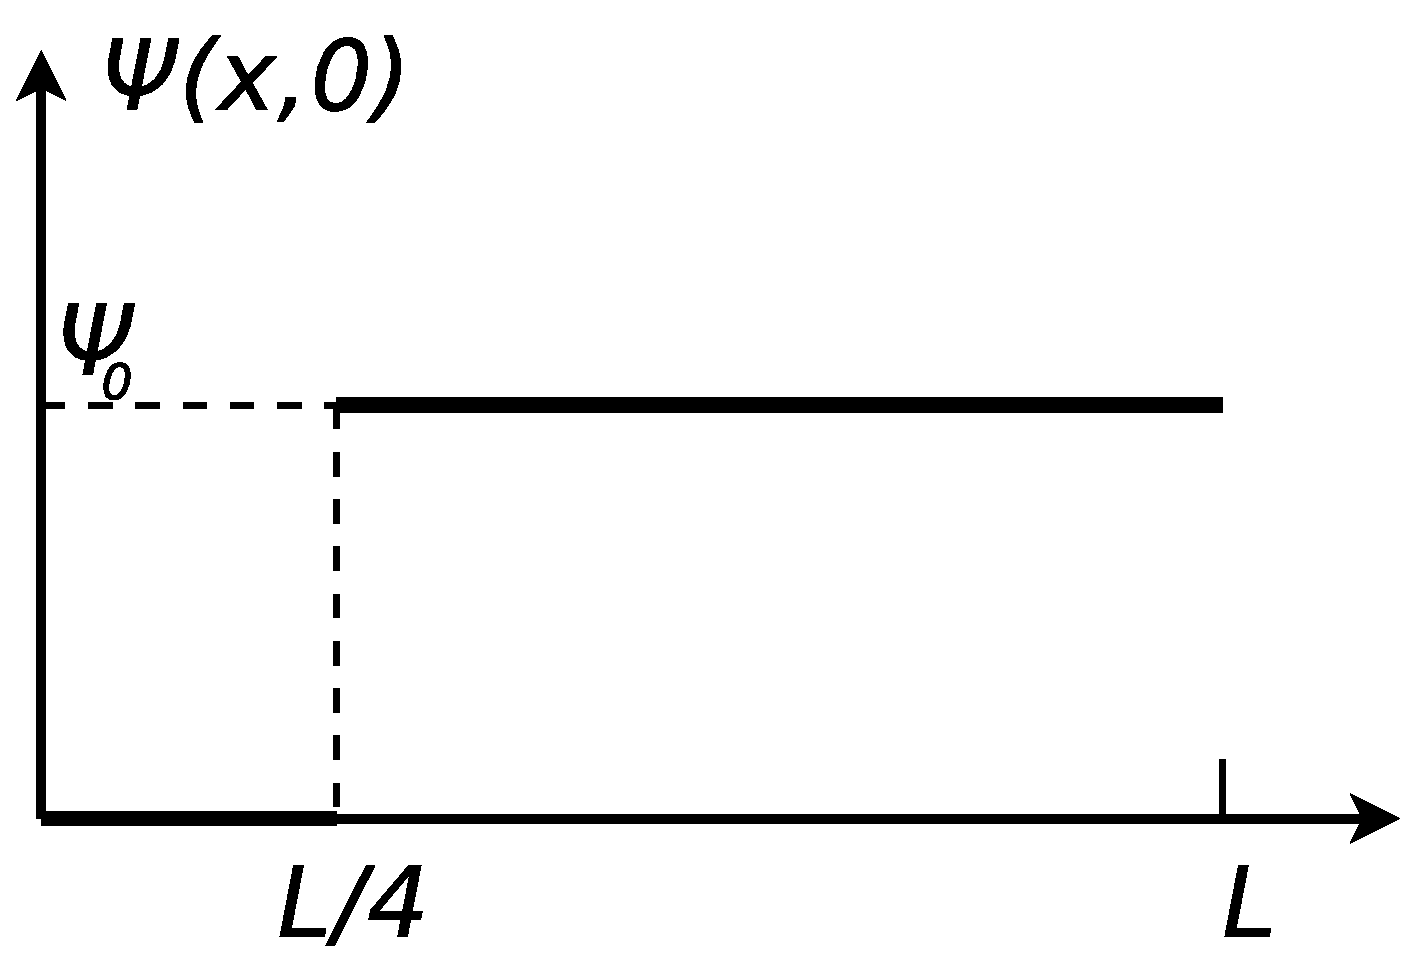
\includegraphics[clip,scale=0.25]{figs/ej1-25}
    \end{figure}

    \begin{enumerate}
        \item Usando el sistema de coordenadas indicado en la figura, halle
        $\Psi(x,t)$.

        \item Graficar $\Psi(x,t)$ para $\omega_{1}t=0,\,\pi$ y $2\pi$.

        \item Si tomara un sistema de coordenadas con el origen en el extremo
        libre de la cuerda, diga qué es lo que cambiaría. ¿Es conveniente ese
        sistema?
    \end{enumerate}

% Ejercicio 9

    \item Considere una cuerda de longitud $L$, siendo $T_{0}$ su tensión y
    $\mu_{0}$ su densidad lineal. Sea $\Phi(x,t)$ la elongación de la cuerda.

    \begin{enumerate}
        \item Escriba la expresión más general que representa un modo normal en
        dicha cuerda, es decir, la expresión más general de una onda
        estacionaria.

        \item Sabiendo que la cuerda tiene un extremo libre y otro fijo, y que
        el sistema de coordenadas con el que trabaja es tal que el extremo libre
        está en $x=0$ y el extremo fijo está en $x=L$, imponga las condiciones
        de contorno y determine las constantes pertinentes.

        \item Usando la relación de dispersión, obtenga las posibles frecuencias
        temporales $\nu_{n}$.

        \item Si $\Phi(x,0)=0$ y $\dot{\Phi}(x,0)=V_{0}\cos\left(\frac{3\pi}{2L}x\right)$,
        siendo $0\le x\le L$, obtenga la amplitud y fase de cada modo y halle
        $\Phi(x,t)$.
    \end{enumerate}

% Ejercicio 10

    \item Dada una cuerda de longitud $L$ y densidad de masa uniforme $\mu$,
    sometida a una tensión $T_{0}$ con ambos extremos fijos, demostrar que si
    $\Phi(x,0)$ y $\dot{\Phi}(x,0)$ son simétricas con respecto al centro de la
    cuerda, los modos con números de onda $k_{p}=2p\pi/L$ no se excitan.

% Ejercicio 11

    \item Considere una cuerda de longitud $L$ sujeta en ambos extremos y
    sometida a una tensión $T_{0}$, que consta de dos tramos: uno de longitud
    $L_{1}$ y densidad de masa uniforme $\mu_{1}$, y otro de longitud
    $L_{2}$ y densidad de masa uniforme $\mu_{2}$.

    \begin{enumerate}
        \item Halle la expresión más general para un modo normal en dicha
        cuerda. Plantee las condiciones de contorno y halle las condiciones que
        deben cumplir los distintos parámetros.

        \item Considere que $L_{1}=3L_{2}$ y que $\mu_{2}=9\mu_{1}$. Hallar los
        modos normales en este caso.
    \end{enumerate}

% Ejercicio 12

    \item Se tiene una cuerda de longitud $L$ y densidad de masa uniforme $\mu$,
    sometida a una tensión $T_{0}$ y fija en ambos extremos. Se tiene además
    que una fuerza de amortiguamiento proporcional a la velocidad de la cuerda
    actúa en cada punto de la misma. Hallar la forma más general de $\Phi(x,t)$.

% Ejercicio 13

    \item Se tiene un tubo de longitud $L$ cerrado en ambos extremos como se
    indica en la figura. El tubo presenta un tabique ubicado en la mitad del
    mismo. De un lado del tabique hay un gas de densidad $\rho_{0}-\Delta$ y del
    otro lado hay un gas de densidad $\rho_{0}+\Delta$ (considere $\Delta\ll\rho_{0}$).
    Todo el gas se encuentra en reposo. A $t=0$ se quita el tabique y se deja
    evolucionar al sistema.

    \begin{figure}[H]
        \centering{}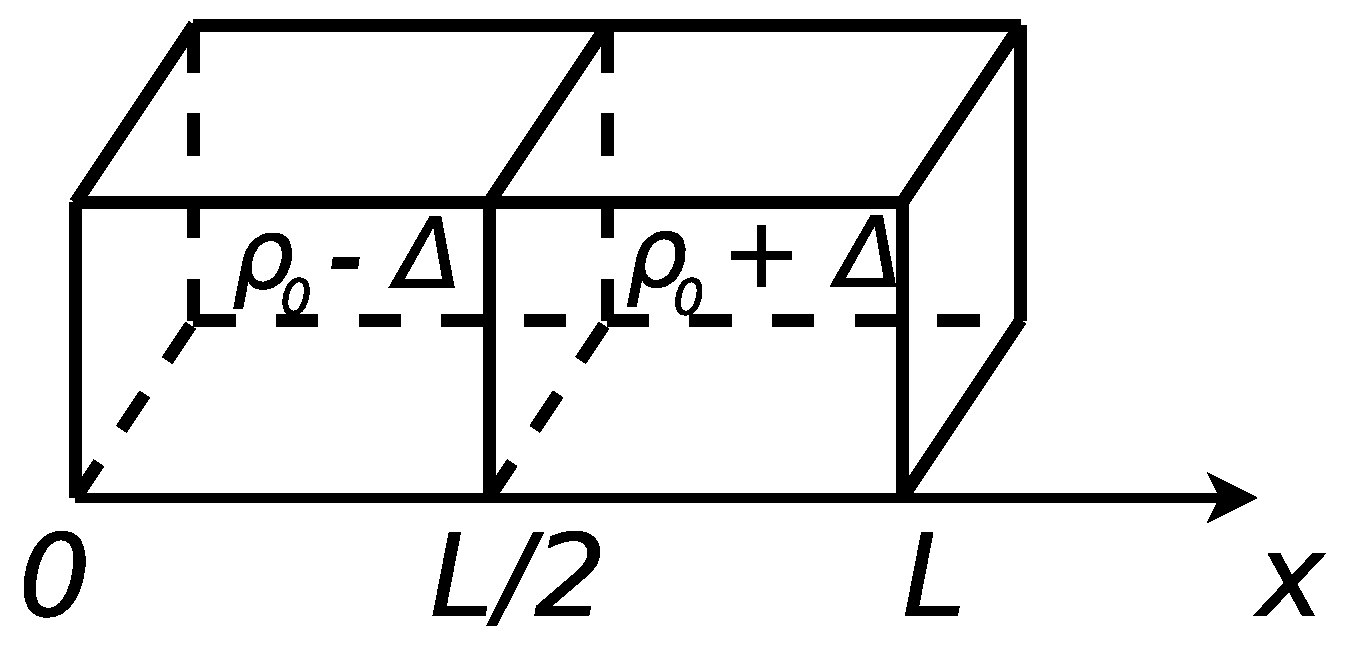
\includegraphics[clip,scale=0.25]{figs/ej1-30}
    \end{figure}

    \begin{enumerate}
        \item Escriba la expresión para un modo normal $\Psi_{n}(x,t)$ en el
        tubo, imponiendo las condiciones de contorno. ¿Cuáles son las longitudes
        de onda permitidas? ($\Psi$ es el desplazamiento de los elementos del
        gas). 

        \item Escriba la expresión de $\rho(x,0)$ y de $\Psi(x,0)$; grafíquelas.
        Sugerencia: hallar $\Psi(x,0)$ a partir de $\rho(x,0)$ usando las
        condiciones de contorno.

        \item Usando las condiciones iniciales, halle $\Psi(x,t)$. Calcule
        $\rho(x,0)$.
    \end{enumerate}

    \begin{description}
        \item [{Datos:}] $\rho_{0}$, $\Delta$, $L$, velocidad del sonido en el
        gas $v_\text{s}$.
    \end{description}

% Ejercicio 14

    \item Se tiene un tubo dividido en dos regiones separadas por un tabique.
    En una de ellas se tiene una presión $P=P_{0}+\Delta p$ (constante). La otra
    región está abierta a la atmósfera, teniendo presión $P_{0}$. A $t=0$ se
    remueve el tabique. Hallar $\delta p(x,t)$, $\Psi(x,t)$ y $\delta\rho(x,t)$.

    \begin{figure}[H]
        \centering{}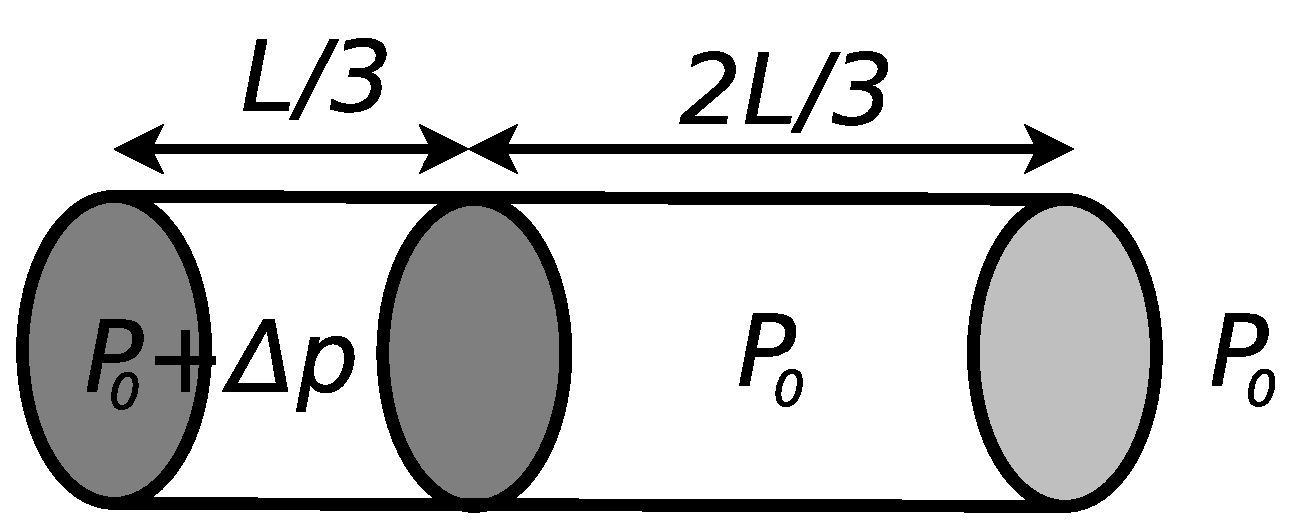
\includegraphics[clip,scale=0.25]{figs/ej1-31}
    \end{figure}

    \begin{description}
        \item [{Datos:}] $P_{0}$, $\Delta p\ll P_{0}$, $L$, $\gamma$ y la
        velocidad del sonido en el gas $v_\text{s}$.
    \end{description}

% Ejercicio 15

    \item Se tiene una cuerda de longitud $L=0,6\unit{\, m}$, fija en sus dos
    extremos, que se encuentra oscilando en uno de sus modos normales como se
    muestra en la figura. La velocidad de propagación de las ondas en dicha
    cuerda es $v=80$ m/s.

    \begin{figure}[H]
        \centering{}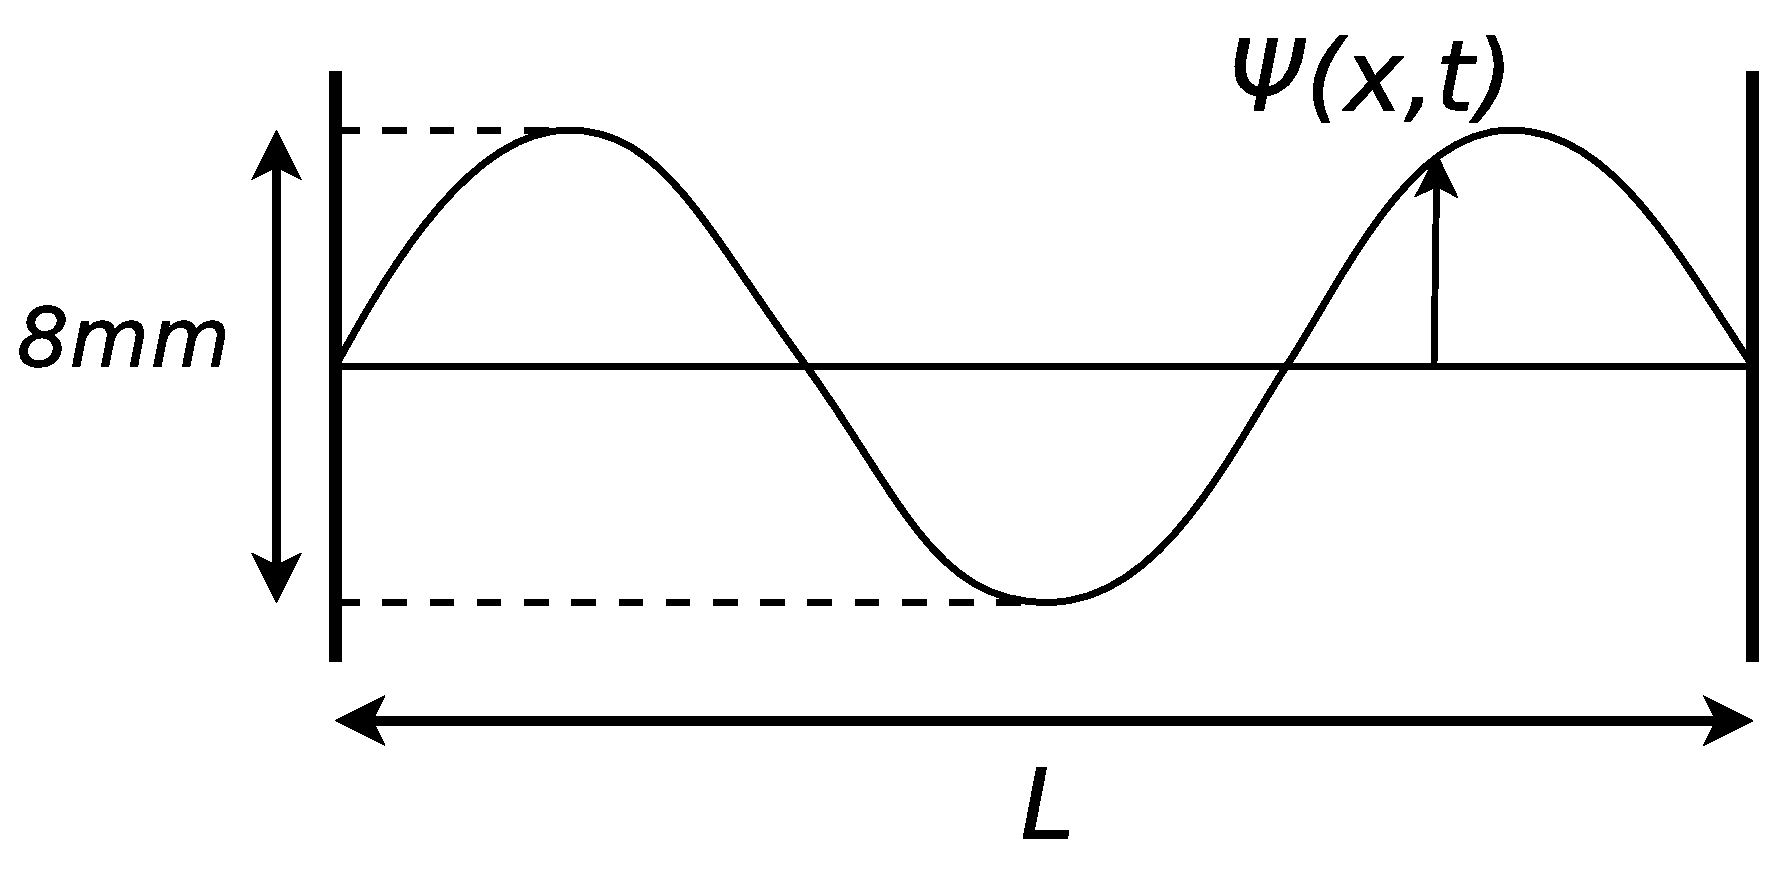
\includegraphics[clip,scale=0.25]{figs/ej1-32}
    \end{figure}

    \begin{enumerate}
    \item Escribir $\Psi(x,t)$ (la elongación en un punto de la cuerda),
    sabiendo que a $t=0$ la elongación de todos los puntos es nula; que la
    amplitud total máxima de la onda es de 8 mm, y que $\dot{\Psi}(L/2,0) > 0$.

    \item Hallar $\Psi_{1}(x-vt)$ y $\Psi_{2}(x+vt)$ tales que
    $\Psi(x,t)=\Psi_{1}(x-vt)+\Psi_{2}(x+vt)$; es decir, escribir a $\Psi(x,t)$
    como la superposición de dos ondas viajeras.
\end{enumerate}

% Ejercicio 16

    \item Se tiene una cuerda de longitud $L=$1 m, con un extremo fijo y uno
    libre, oscilando en el modo normal que se muestra en la figura. La
    velocidad de propagación de las ondas en dicha cuerda es $v=80$ m/s, y el
    desplazamiento de las partículas a $t=0$ es el máximo posible para este
    modo, siendo $\Psi(L,0)>0$. La amplitud total máxima es de 8 mm.

    \begin{figure}[H]
        \centering{}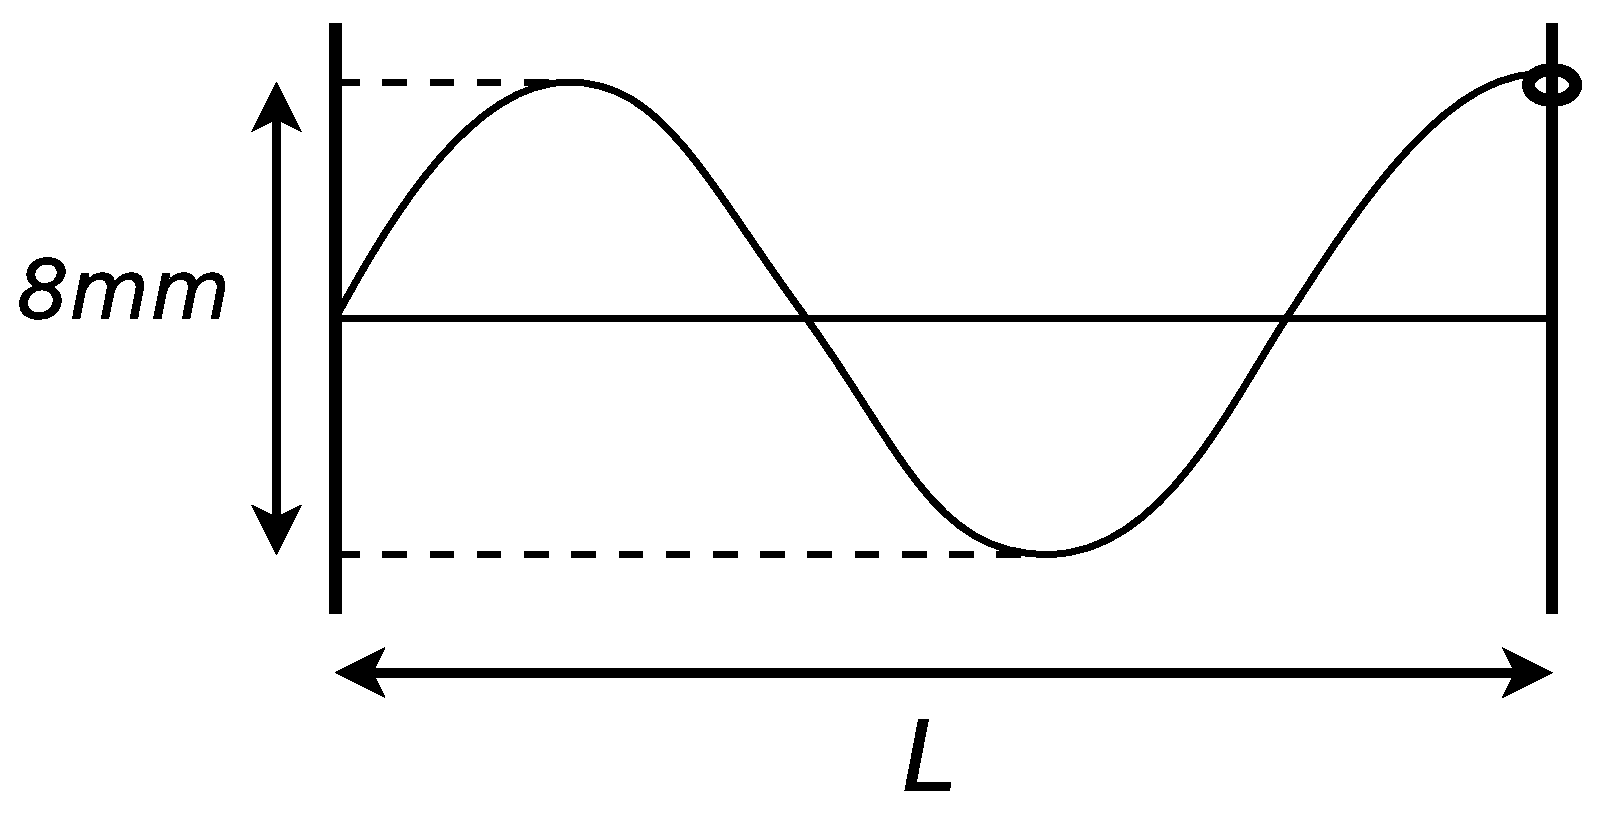
\includegraphics[clip,scale=0.25]{figs/ej1-33}
    \end{figure}

    \begin{enumerate}
        \item Resolver, para esta situación, todo lo pedido en el problema
        anterior. 

        \item Si ahora la cuerda está oscilando en un modo normal arbitrario
        $n$, con las mismas condiciones iniciales dadas arriba, repetir (a)
        (expresar en función de $n$).
    \end{enumerate}

\section*{Ecuación de Klein-Gordon}

% Ejercicio 17

    \item Considere un arreglo lineal de péndulos acoplados excitados cuyo
    extremo inferior está en $z=0$ y unidos a una pared rígida en $z=L$, como
    se muestra en la figura.

    \begin{figure}[H]
        \centering{}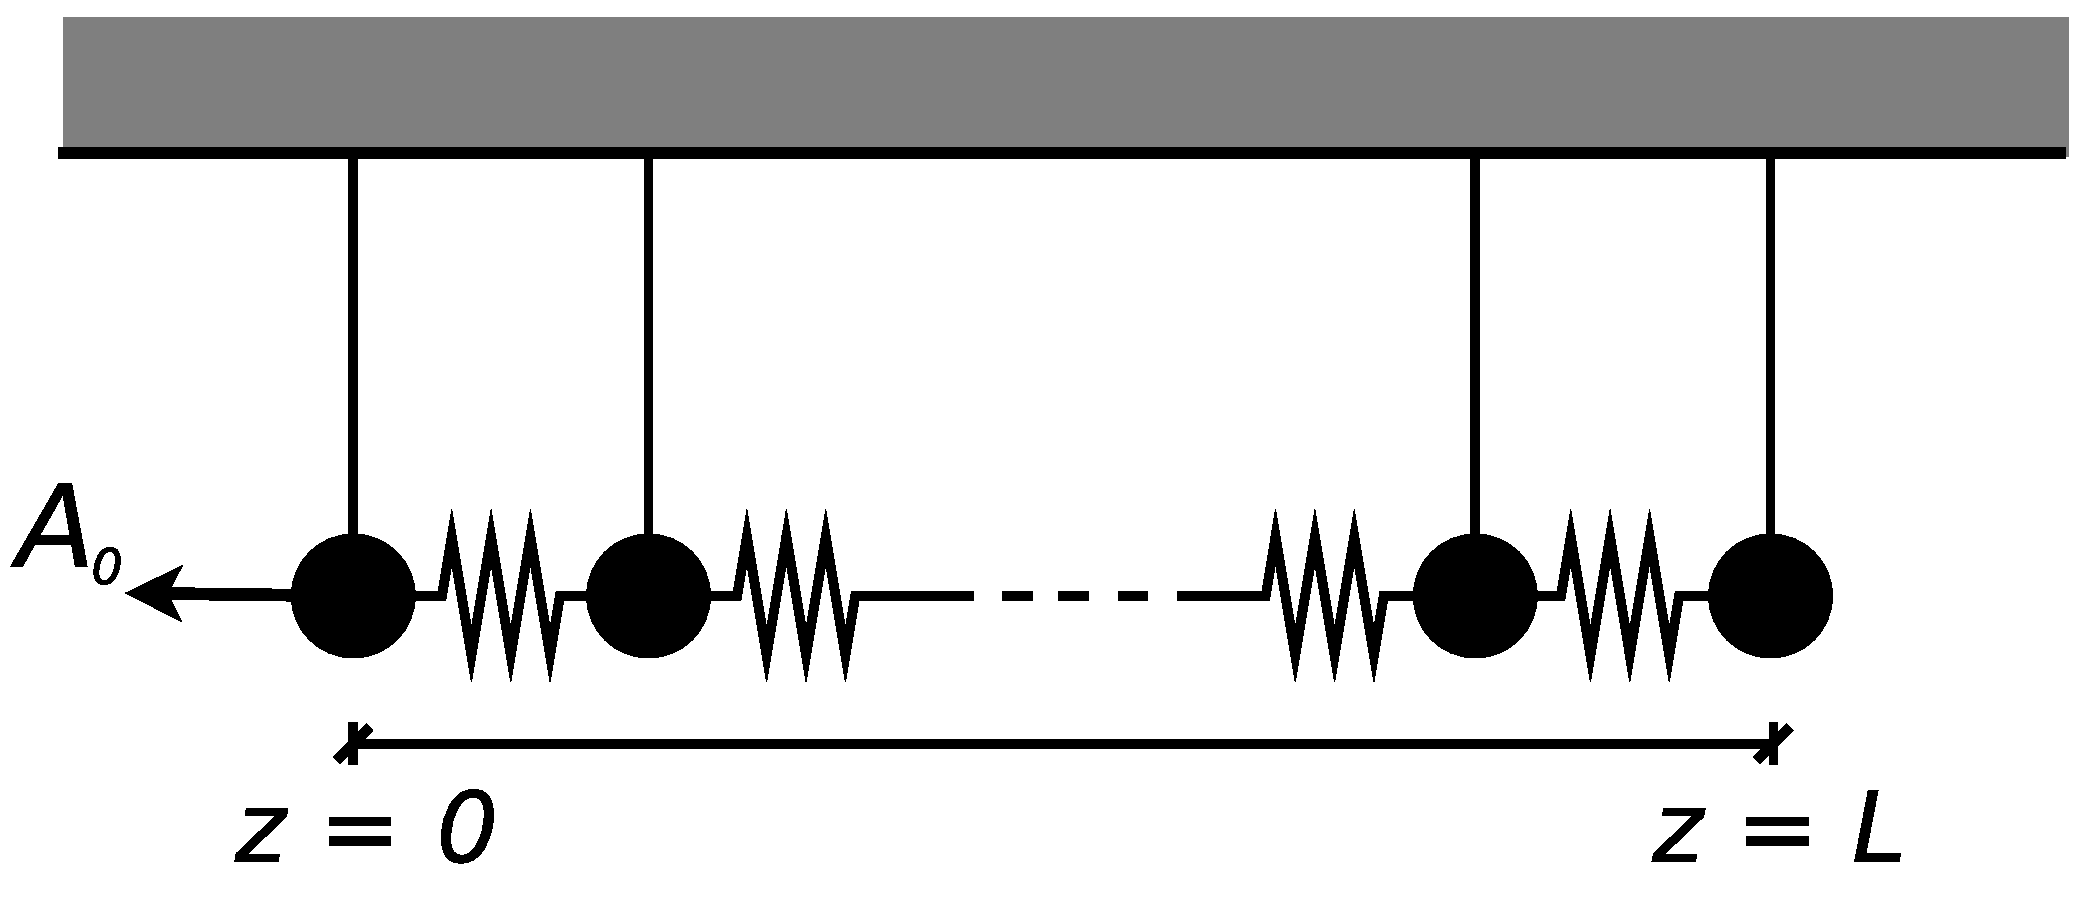
\includegraphics[clip,scale=0.25]{figs/ej1-15}
    \end{figure}

    Se aplica una fuerza externa en función del tiempo a la primera masa
    ($z=0$), de forma tal que se conoce su amplitud
    $\Psi(0,t)=A_{0}\cos(\Omega t)$. Halle el movimiento estacionario del
    sistema y discuta las hipótesis que hace. Compare con el caso de extremo
    derecho fijo a una pared (o sea: agregando un resorte a la derecha de la
    última masa y uniéndolo a la pared).

% Ejercicio 18

    \item Considere un sistema de péndulos acoplados con un cambio brusco en
    $\omega_{0}^{2}$ en $z=L$, según se esquematiza en la figura. Halle el
    movimiento estacionario del sistema y discuta las hipótesis quee hace.

    \begin{figure}[H]
        \centering{}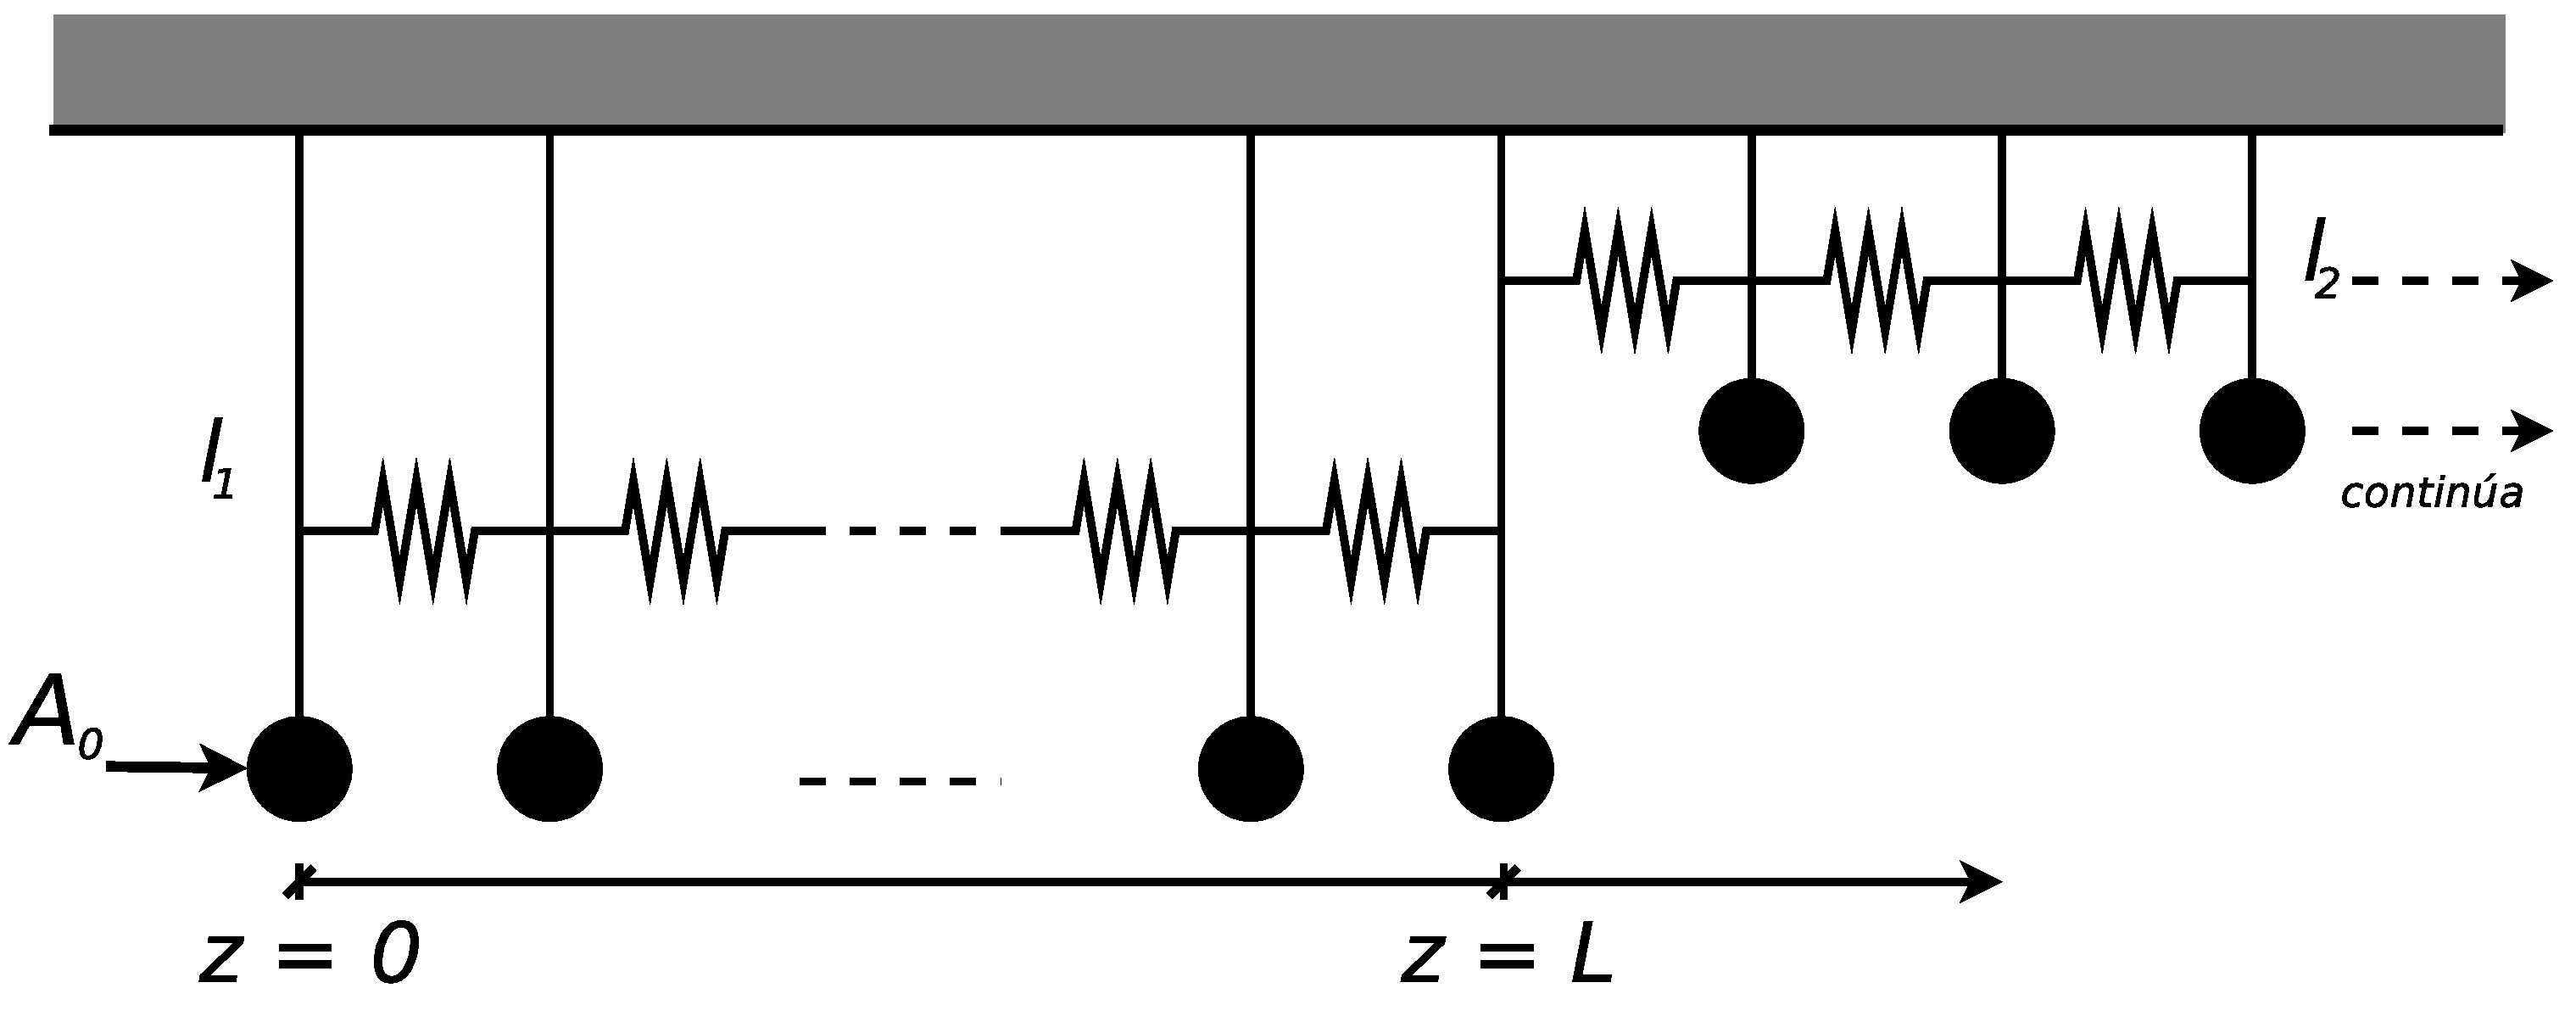
\includegraphics[clip,scale=0.25]{figs/ej1-16}
    \end{figure}

% Ejercicio 19
    
    \item Para el sistema esquematizado en la figura, calcule $\Psi_{n}(t)$, si
    $\Omega<\omega_\text{min}$.

    \begin{figure}[H]
        \centering{}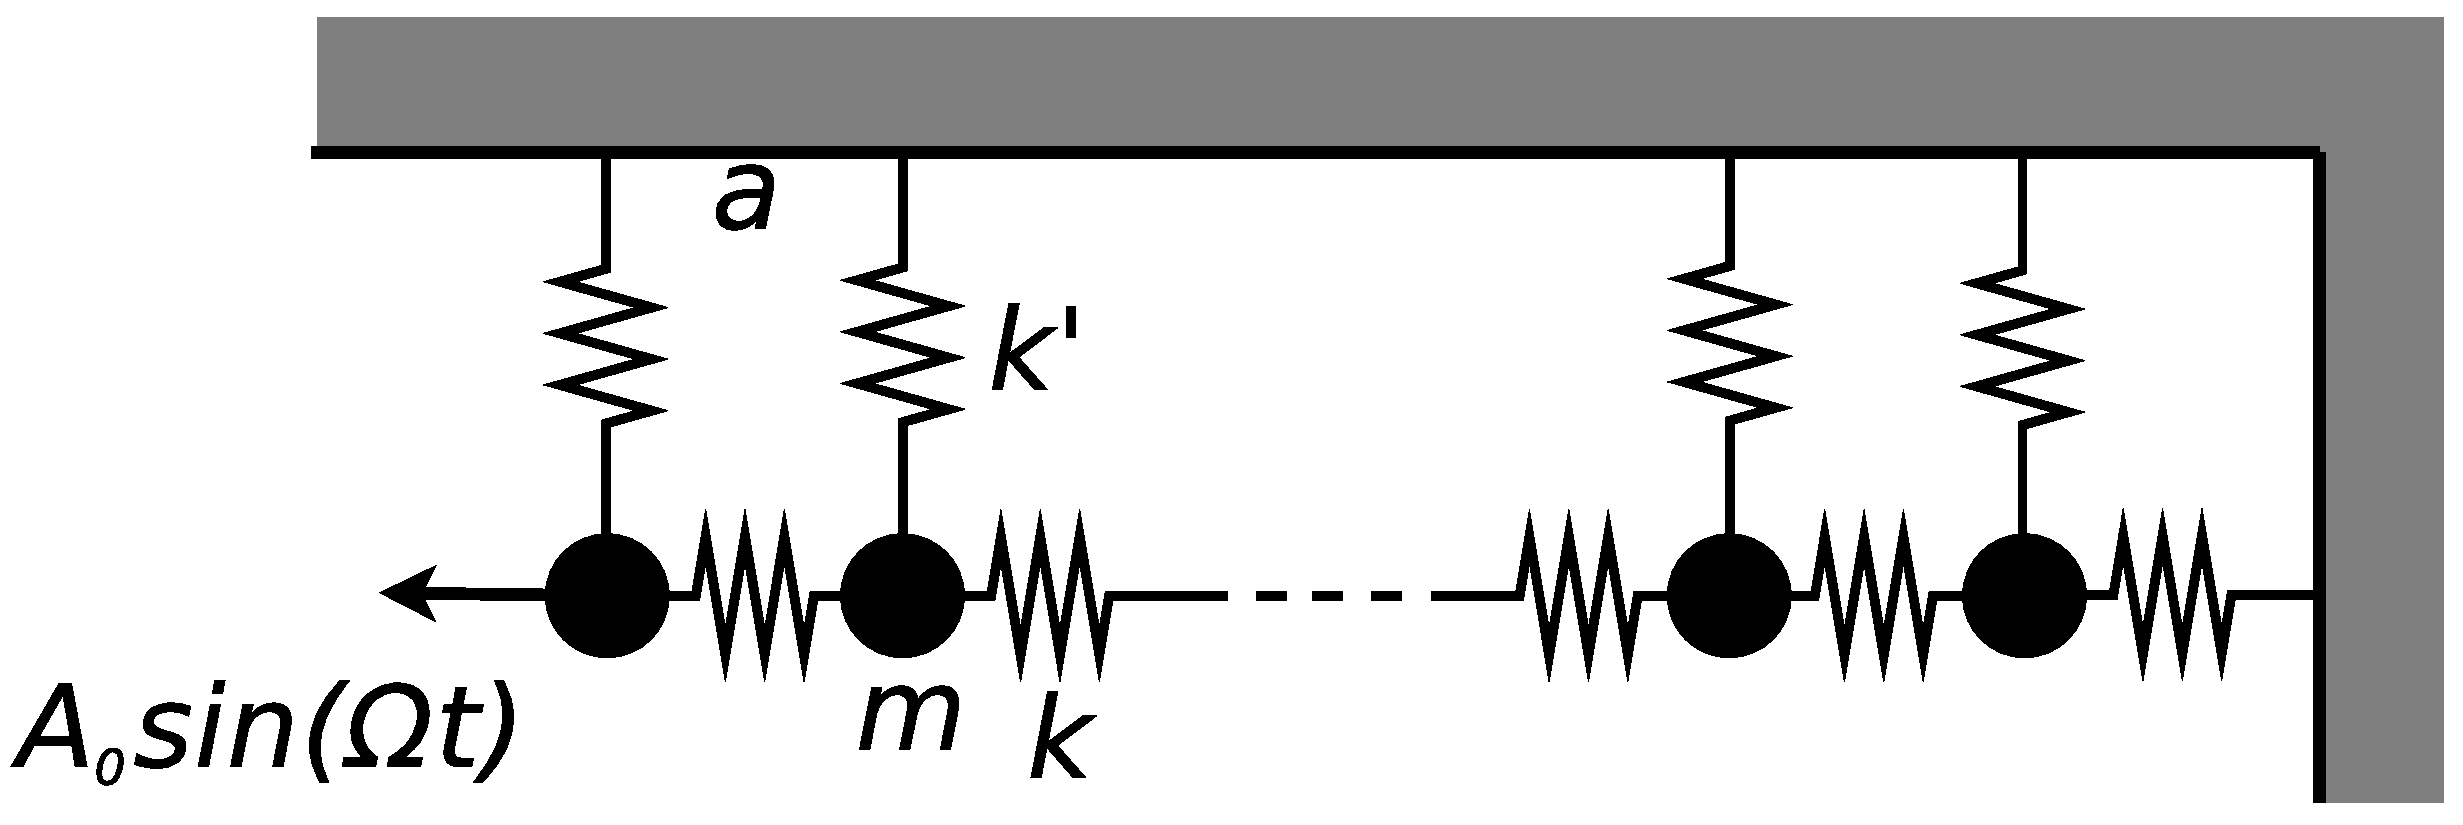
\includegraphics[clip,scale=0.25]{figs/ej1-17}
    \end{figure}


\end{enumerate}

\end{document}
